\newpage
\section{Sistema Pipeline}
Una architettura pipeline è una tipologia di soluzione che viene implementata internamente nei processori per permettere l'esecuzione parallela di più istruzioni.
Per comprendere meglio cosa si intende per esecuzione parallela di più istruzioni, andiamo a considerare la strutturazione interna del flusso di esecuzione di una normale istruzione. L'esecuzione si divide nelle seguenti fasi (visualizzabili anche alla figura [\ref{img:pipe}]):
\begin{itemize}
    \item \textbf{Istruction Fetch (IF)}: Ovvero il prelievo dell'istruzione dalla memoria;
    \item \textbf{Decode (DEC)}: Decodifica ed interpretazione dell'istruzione;
    \item \textbf{Execute (EX)}: Esecuzione effettiva dell'istruzione;
    \item \textbf{Memory write (MW)}: Effettuo il prelievo dei dati all'interno della memoria;
    \item \textbf{Register write (RW)}: Inserisco i dati che mi interessano dai registri, in memoria. 
\end{itemize}

\begin{figure}
    \centering
    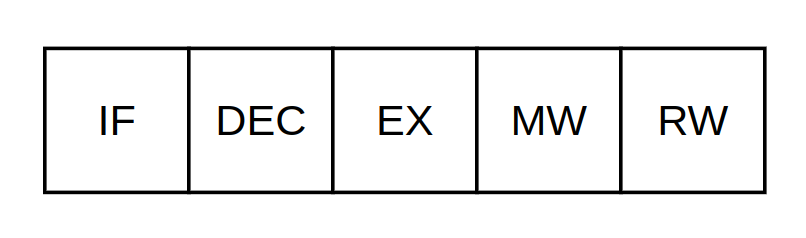
\includegraphics[width=.5\textwidth]{img/Pipeline.png}
    \caption{Architettura classica pipeline (ordine di esecuzione fasi)}\label{img:pipe}
\end{figure}

Definito il flusso di esecuzione di un' istruzione, l'architettura pipeline cerca di eseguire le fasi di un' istruzione in maniera del tutto separata, in modo da poter eseguire più fasi di istruzioni differenti. Per capire meglio questo concetto facciamo un esempio:
Devo eseguire un programma che ha 5 istruzioni, allora parto con l'esecuzione della prima fase, che preleverà l'istruzione i1, una volta prelevata, l'istruzione i1 passa alla fase di decode, mente, allo stesso istante, viene caricata l'istruzione i2 (quindi viene effettuata la Istruction Fetch dell'istruzione successiva mentre viene decodificata la precedente). Se eseguiamo tale procedura per tutte le fasi noteremo che ad ogni impulso di clock (a regime), il processore darà un risultato, quindi non ci sarà bisogno di eseguire tutte le istruzioni una per volta, poichè la suddivisione delle fasi ne permette un' esecuzione "parallela" (o meglio dire pipeline).

Per fare in modo di isolare l'esecuzione delle varie fasi, tra i vari blocchetti saranno presenti dei registri, che permettono di conservare lo stato su cui una determinata fase sta lavorando (come le architetture pipeline in elettronica [\ref{img:pipe-reg}]). 

\begin{figure}
    \centering
    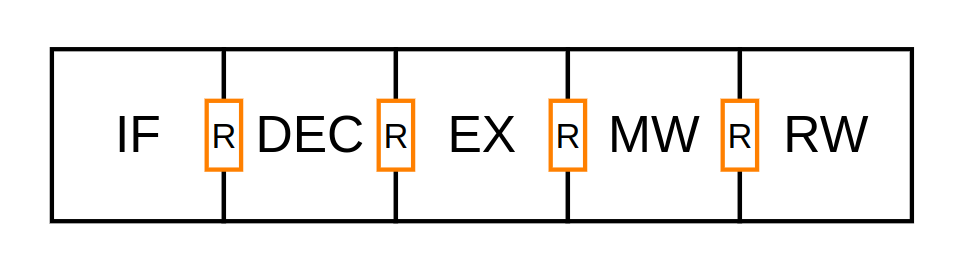
\includegraphics[width=.5\textwidth]{img/Pipe-reg.png}
    \caption{Architettura classica pipeline con registri}\label{img:pipe-reg}
\end{figure}

Un'architettura di questo tipo, però, richiede una serie di ipotesi, ovvero:
\begin{itemize}
    \item Divisione di parte dati e parte istruzioni (altrimenti dovrei gestire anche dei conflitti tra l'istruction fetch e la register/memory write);
    \item Le memorie devono avere degli accessi molto veloci: ad ogni colpo di clock viene prelevata un'istruzione e potenzialmente scritto un risultato.
    \item Le operazioni artimetico-logiche devono essere effettuate prevalentemente tra i registri interni del processore;
    \item Le istruzioni devono avere tutte lunghezza fissa;
\end{itemize}

Guardando le ipotesi possiamo capire che alcune tipologie di operazioni, che solitamente effettuevamo sul processore motorola, ora dovranno essere scompattate in varie operazioni. Un esempio classico è il comando \lstinline|ADD VAR,D1|, che utilizzava l'indirizzamento diretto per il prelievo dell'operando dalla memoria. In questo caso, però, l'indirizzamento diretto non è possibile, poichè si andrebbe ad invalidare un'ipotesi, ovvero, la lunghezza fissa dell'istruzione (che dovrebbe poi contenere l'indirizzo di memoria). Pertanto non sono previsti tutti i modi di indirizzamento.

Per comprendere meglio la problematica, consideriamo di avere un prelievo dalla memoria con un'architettura a 16-bit, ma con il memory address ed il memory buffer a 32-bit. Pertanto il seguente comando non sarebbe possibile: \lstinline|MOVE VAR,D0|; poichè richiederebbe il prelievo dell'indirizzo di memoria da 32-bit dalla memoria, ma per effettuare tale operazione, avendo solo 16 bit, avrei bisogno di due istruzioni che caricano, una i primi 16-bit e l'altra i restanti 16. Tale suddivisione, però non viene fatta dal programmatore, ma dal compilatore. Ci sono varie istruzioni che sono come la MOVE, tali istruzioni sono dette pseudo-istruzioni, poichè il compilatore andrà a suddividerle in più operazioni differenti al fine di raggiungere il risultato desiderato.

Questa cosa ci permette di capire, a questo punto, la suddivisione tra architettura di tipo CISC e architetture di tipo RISC. Le architetture di tipo CISC permettono l'esecuzione di istruzioni che sono più articolate, ma a costo di una complessità architetturale maggiore, mentre nelle architetture RISC, data la semplicità dell'architettura, le tipologie di operazioni che si possono effettuare sono ridotte ma più veloci.

\subsection{Modelli di sistemi pipeline}
Il sistema pipeline, dato il suo sistema di funzionamento, può introdurre varie tipologie di problematiche. Negli anni si sono sviluppate varie tipologie di soluzioni differenti.
Le principali architetture con cui si va a contatto al giorno d'oggi sono:
\begin{itemize}
    \item \textbf{MIPS}: Tipologia di ISA sviluppata da Patterson che poi ha venduto, per cui ora la sua implemetazione è proprietaria;
    \item \textbf{RISC-V}: Tipologia di ISA molto simile al MIPS, ma open-source;
    \item \textbf{ARM}: Tipologia di ISA proprietaria, utilizzatissima in svariati amiti (particolarmente in quello industriale), la cui implementazione è proprietaria;
\end{itemize}

Nel caso particolare di questo corso, andremo a vedere il funzionamento del RISC-V facendo riferimento sempre al MIPS, per cui saranno queste le due tipologie di architetture che si andranno ad approfondire.

Le principali problematiche che bisogna affrontare all'interno di un architettura pipeline sono le seguenti:
\begin{itemize}
    \item \textbf{Interruzioni}: Quando bisogna gestire un' interruzione la gestione dell'architettura pipe si complica, poichè bisogna capire chi ha interrotto e bisogna salvare lo stato di tutte le istruzioni che stanno eseguendo, che risulta una cosa molto onerosa e complicata;
    \item \textbf{Concorrenza sui registi}: Se due istruzioni, devono utilizzare un'informazione presente nello stesso registro ad esempio: R1 = R2+R3; R0=R1+R4;  Notiamo che per eseguire la seconda istruzione vi è bisogno del completamento della prima, ma il risultato effettivo viene scritto solo alla fine del ciclo, per cui si potrebbe incorrere in vari errori;
    \item \textbf{Salti}: Quando devo effettuare un salto, se considero il caso condizionato, non so a quale ramo andrò a saltare, è quindi più complicato capire quale sarà l'istruzione successiva da eseguire;
    \item \textbf{Gestione delle pipe multiple}: ho molteplici pipe di esecuzione, che quindi richiede una loro gestione per prevenire eventuali conflitti;
\end{itemize}

Una delle problematiche che maggiormente incide è quella riguardante il salto, poichè, dato che non conosco quale sia l'istruzione successiva, vado a bloccare la pipe appena noto che ho un'istruzione di salto, ed appena è verificata la condizione, vado a prelevare tale istruzione dalla memoria. Però questa soluzione risulta molto inefficiente, poichè introduce dei periodi in cui la pipe rimane in stallo. Difatti, una soluzione che è stata trovata è quella della branch prediction, per cui vado a processare le istruzioni successive, cercando di prevedere quale sarà il branch da eseguire, solo nel caso in cui mi accorgo che sto sbagliando vado ad effettuare il blocco della pipe, altrimenti continuo con la normale esecuzione del programma.

\subsection{Architettura del MIPS}
Il MIPS (Microprocessor without Interlocked Pipelined Stages) è una tipologia di architettura Pipelined di tipo RISC.
Nel precedente capitolo abbiamo visto le fasi di esecuzione di un'architettura pipelined generale [\ref{img:pipe}], però, nel caso del MIPS, tali fasi variano leggermente. Difatti il MIPS è caratterizzato dalle seguenti fasi:
\begin{itemize}
    \item \textbf{Istruction Fetch}: Prelievo dell'istruzione dalla memoria e incremento del program counter;
    \item \textbf{Decode}: Si vanno a prelevare gli operandi dall'istruction file e si preparano i segnali di controllo per la fase di esecuzione;
    \item \textbf{Execute}: Esecuzione delle operazioni logico-aritmetiche pilotate dai segnali della fase di decode precedente;
    \item \textbf{Memory}: Vado a leggere o scrivere qualcosa dalla memoria e gestione dei Salti;
    \item \textbf{Write Back}: Accedo in scrittura al register file per scrivere i risultati ottenuti;
\end{itemize}

Come per tutte le architettura pipelined, anche il MIPS richiede che tra le varie fasi vi siano dei registri che conservino lo stato dell'operazione.
Il MIPS, pertanto, presenta vari casi di conflitto che richiedono delle ipotesi sul sistema stesso. Tali ipotesi sono:
\begin{itemize}
    \item \textbf{Velocità della memoria}: La memoria che sarà utilizzata dal MIPS sarà acceduta molto frequentemente (precisamente 5 volte in più rispetto al caso senza pipe);
    \item \textbf{Concorrenze sulla memoria}: Presenza di due memorie, una per le istruzioni ed una per i dati. Tali memorie vengono previste per evitare la concorrenza tra la fase di fetch (prelievo dell'istruzione dalla memoria) e la fase di MEM (lettura o scrittura dalla memoria);
    \item \textbf{Concorrenza sui registri}: Si prevede che la fase di Decode sia eseguita nella seconda parte del ciclo clock, mentre la fase di write back nella prima parte del ciclo di clock. Tale presupposizione viene fatta, per evitare la concorrenza sui registri che interessano l'operazione, e quindi evitare conflitti indesiderati.
\end{itemize}

\subsubsection{Fase di Fetch}
La fase di fetch è caratterizzata da 2 principali operazioni, la fase di prelievo dell'indirizzo e la fase di incremento del program counter. Pertanto la sua parte architetturale è formata dalle componenti:
\begin{itemize}
    \item \textbf{ADD}: Strumento aritmetico per l'incremento del program counter (differente dal componente di ALU);
    \item \textbf{MUX}: Seleziona se considerare l'indirizzo di memoria successivo del program counter o un registro di memoria dettato dalla fase di MEM;
    \item \textbf{PC}: Registro program counter;
    \item \textbf{Istruction Memory}: Vado a prelevare l'istruzione da eseguire dalla memoria;
\end{itemize}

\subsection{Fase di Decode}
Nella fase di Decode, il MIPS, va a decodificare ed interpretare il comando. Le parti che compongono l'architettura della fase di decode sono:
\begin{itemize}
    \item \textbf{Registers}: Registri interni del processore che possono essere pilotati sia in lettura che in scrittura tramite dei segnali esterni (contenuti nella sotto-architettura);
    \item \textbf{Sign-extend}: Blocco di estensione con segno dei possibili valori immediati contenuti nell'istruzione;
\end{itemize}

\subsection{Fase di Execute}
Nella fase Execute viene eseguita effettivamente l'istruzione. La parte architetturale è composta da vari componenti interessanti
\begin{itemize}
    \item \textbf{Add}: Strumento che viene utilizzato per calcolare un eventuale offset rispetto ad un valore;
    \item \textbf{Shift left 2}: Vado a moltiplicare per 4 il valore per cui voglio saltare (in modo da saltare a 4 indirizzi più avanti);
    \item \textbf{ALU}: Strumento di calcolo aritmetico;
    \item \textbf{Multiplexer}: Vedo se devo selezionare il dato immediato o un secondo dato proveniente da un registro;
\end{itemize}

\subsection{Fase di Mem}
Nella fase di memorizzazione vado ad interagire con la memoria per effettuare o operazioni di lettura o operazioni di scrittura
La sua architettura è composta principalmente dal singolo elemento di accesso alla memoria dati

\subsection{Fase di Write Back}
In tale fase vado a verificare cosa bisogna scrivere all'interno dei registri interni. Il componente che meglio indica il suo funzionamento è il multiplexer finale che serve per specificare se il dato da caricare all'interno dei registri sia il risultato dell'ALU o qualche valore proveniente dalla memoria

\subsection{Registri Intermedi}
I registri che sono posti tra una fase e l'altra della pipeline sono molto più complessi di quel che si crede. Essi non contengono solo dati informativi (operandi e risultati), ma contengono anche: traccia dell'operazione da effetture, destinazione del risultato ecc. 
L'architettura e le componenti di cui si è parlato sopra, quindi, sono solo una parte di quello che è effettivamente stato realizzato sull'hardware del dispositivo.
La schematizzazione che abbiamo fatto ci permette di capire bene il funzionamento di un sistema pipeline senza entrare troppo nei dettagli della sua implementazione hardware

\subsection{Gestione dei Salti}
L'architettura pipeline ha una criticità di cui abbiamo già attentamente discusso in precedenza, i salti.
Quando sopraggiunge un istruzione di salto, riusciamo a captare che è così solo nella fase di esecuzione dell'istruzione, e quindi, se dovessimo aggiustare il PC seguendo tutta la pipe, dovremmo aspettare la fase di write back. Ma per evitare tale situazione, andiamo a retroazionare la fase di esecuzione con la fase di Istruction Fetch. Tale retroazione permette di capire quando e dove poi si andrà a saltare. Ciò però deve prevedere il sacrificio o l'introduzione di un istruzione "vittima", tale istruzione sarà eseguita indipendentemente a dove si andrà a saltare. Tale istruzione è la no-operation (NOP), che viene inserita subito dopo la JMP per evitare la perdita di eventuali istruzioni utili.
Tale soluzione è molto buona quando lavoro con il MIPS, poichè questo è caratterizzato dalla sua particolare pipe molto corta (e quindi molto RISC), ma nei processori più moderni, posso avere delle pipe molto più profonde ed articolate. Una soluzione alternativa a quella proposta precedentemente è quella di utilizzare la branch-prediction

\subsubsection{Branch prediction}
La branch prediction è una tecnica che cerca di prevedere a quale ramo un istruzione di salto condizionato possa saltare. Tale tecnica valuta le prestazioni in base a quanto si possa "perdere" in termini di efficienza (ricaricare il branch corretto rispetto a quello predetto).
Per capire bene questa cosa andiamo a considerare il seguente pseudocodice:
\begin{lstlisting}[language=C]
for (int i = 0; i < N; i++){
    for (int j = 0; j < N; j++){
        operazioni
    }
}
\end{lstlisting}

Tali for prevedono un controllo iniziale sulla variabile. Vedendo come sono strutturati tale controllo prevede l'esecuzione del ramo else una sola volta (guardando il for interno) ogni N passi.
I modi pre prevedere il branch possono essere vari, e possono essere descritti mediante degli appositi automi a stati finiti. Un primo approccio molto basilare è quello di andare a cambiare il branch da caricare successivamente ad ogni errore di decisione e quindi eseguire le operazioni descritte dall'automa [\ref{img:automa-semplice}].

\begin{figure}[!ht]
    \centering
    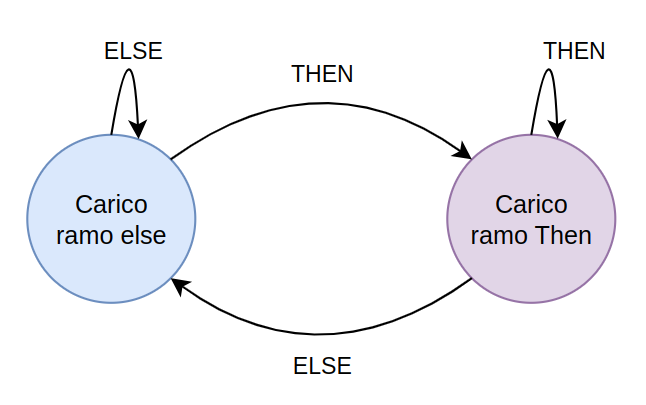
\includegraphics[width=.5\textwidth]{img/automa-semplice.png}
    \caption{Automa della branch prediction base}\label{img:automa-semplice}
\end{figure}

Tale soluzione, però, guardando al nostro caso, non è proprio ottimale, poichè per quel singolo fail che avviene ad ogni N interazioni dovrò assorbirmi 2 fault. Per evitare tale condizione, e quindi rendere la persistenza più forte, vado a costruire un automa a 4 stati che mi permette di rendere la condizione di "cambio del branch" più solida, poichè solo in caso di due fault successivi (fault = errore nel riconoscere il branch giusto), allora cambio il mio branch effettivo. L'automa che meglio spiega tale principio è quello visualizzabille all'immagine [\ref{img:automa-complesso}]

\begin{figure}[!ht]
    \centering
    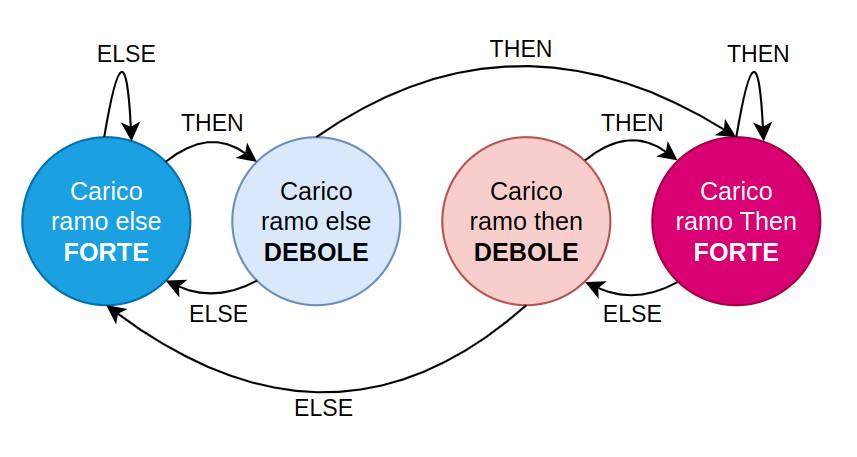
\includegraphics[width=.5\textwidth]{img/automa-complesso.png}
    \caption{Automa della branch prediction avanzato}\label{img:automa-complesso}
\end{figure}

\section{Architetture Superscalari}
L'utilizzo delle pipe porta dei vantaggi non in termini di attraversamento di una istruzione, che rimane invariato, ma in termini di produttività. Per ottenere prestazioni ancora migliori, è possibile realizzare un'architettura con più pipe che eseguono diverse istruzioni in parallelo, così da aumentare la produttività del sistema. Una tale architettura viene chiamata \textbf{Superscalare}. Tuttavia, questa introduce delle problematiche che vanno necessariamente risolte, queste sono:
\begin{enumerate}
    \item Le pipe devono condividere un unico accesso in memoria comune per il prelievo delle istruzioni. In altre parole, anche in presenza di più pipe tutte devono leggere dalla stessa memoria. Questo può creare un collo di bottiglia, perché solo una pipeline alla volta può leggere da lì.
    \item Se le pipe non sono del tutto indipendenti ma condividono delle stazioni, nascono dei problemi di conflitto nell'utilizzo delle unità funzionali condivise. Se due pipeline vogliono usare la stessa unità (ad esempio, la ALU) allo stesso momento, nasce un collisione e una delle due deve aspettare. Questo riduce l'efficienza.
\end{enumerate}

\subsection{Gestione delle Collisioni}
La \textbf{gestione delle collisioni} nella architetture superscalari avviene completamente in hardware. Per comprendere al meglio come un processore con una tale architettura gestisca il problema, introduciamo un esempio. Supponiamo che la CPU sia in grado di realizzare addizione e moltiplicazione in floating point. Come possiamo immaginare, alcune delle operazioni presenti nell'addizione potrebbero essere richieste anche dalla moltiplicazione (e viceversa), mappiamo dunque all'interno di una tabella le diverse operazioni necessarie a completare le due [\ref{tab:mul} e \ref{tab:add}].

\begin{table}[!h]
\centering
\begin{tabular}{|l|c|c|c|c|c|c|c|}
\hline
         & 1 & 2 & 3 & 4 & 5 & 6 & 7 \\
\hline
Ex Add   & X &   &   &   &   &   &   \\
\hline
Mult     &   & X & X &   &   &   &   \\
\hline
Man Add  &   &   & X & X &   &   &   \\
\hline
Renorm   &   &   &   &   & X &   & X \\
\hline
Round    &   &   &   &   &   & X &   \\
\hline
Shift A  &   &   &   &   &   &   &   \\
\hline
Lead 1   &   &   &   &   &   &   &   \\
\hline
Shift B  &   &   &   &   &   &   &   \\
\hline
\end{tabular}
\caption{7 stadi richiesti dalla moltiplicazione.}
\label{tab:mul}
\end{table}

\begin{table}[!h]
\centering
\begin{tabular}{|l|c|c|c|c|c|c|c|c|c|}
\hline
         & 1 & 2 & 3 & 4 & 5 & 6 & 7 & 8 & 9 \\
\hline
Ex Add   & X &   &   &   &   &   &   &   &   \\
\hline
Mult     &   &   &   &   &   &   &   &   &   \\
\hline
Man Add  &   &   &   & X &   &   &   &   &   \\
\hline
Renorm   &   &   &   &   &   &   &   &   & X \\
\hline
Round    &   &   &   &   &   &   &   & X &   \\
\hline
Shift A  &   & X & X &   &   &   &   &   &   \\
\hline
Lead 1   &   &   &   &   & X &   &   &   &   \\
\hline
Shift B  &   &   &   &   &   & X & X &   &   \\
\hline
\end{tabular}
\caption{9 stadi richiesti dall'addizione.}
\label{tab:add}
\end{table}

L'introduzione di tali tabelle semplifica notevolmente la scrittura del \textbf{vettore delle collisioni}, ovvero un particolare vettore binario utilizzato dal compilatore per gestire il problema dei conflitti tra pipe. Poniamoci nell'ipotesi semplificativa di due sole pipe, in modo da visualizzare pù facilmente il processo. Per ricavare il vettore, è sufficiente sovrapporre le tabelle delle operazioni che vogliamo eseguire, opportunamente shiftate a seconda di quale delle due sia eseguita prima. Ad esempio, se vogliamo eseguire una moltiplicazione X e al ciclo di clock successivo un'altra moltiplicazione Y, la sovrapposizione delle tabelle fornisce il seguente risultato [\ref{tab:collision}].

\begin{table}[!h]
\centering
\begin{tabular}{|l|c|c|c|c|c|c|c|}
\hline
         & 1 & 2 & 3 & 4 & 5 & 6 & 7 \\
\hline
Ex Add   & X & Y &   &   &   &   &   \\
\hline
Mult     &   & X & XY & Y &   &   &   \\
\hline
Man Add  &   &   & X & XY & Y &   &   \\
\hline
Renorm   &   &   &   &   & X & Y & X \\
\hline
Round    &   &   &   &   &   & X & Y \\
\hline
Shift A  &   &   &   &   &   &   &   \\
\hline
Lead 1   &   &   &   &   &   &   &   \\
\hline
Shift B  &   &   &   &   &   &   &   \\
\hline
\end{tabular}
\caption{Collisioni tra due moltiplicazioni sfasate di 1 ciclo di clock.}
\label{tab:collision}
\end{table}
La tabella evidenzia come le due operazioni, eseguite secondo la tempificazione descritta, presentano delle collisioni al tempo 3 e 4 (presenza contemporanea di X e Y). Il corrispondente vettore delle collisioni sarà dunque 0011000. \MakeUppercase{è} fondamentale ribadire che il vettore si limita solamente a segnalare la presenza di una collisione (1 nella stringa), ma ciò non ha niente a che vedere con le fasi della pipeline. In altre parole, se nella stringa c'è un 1 nella terza posizione, questo NON significa che la collisione riguarda la terza fase.
\\
\\
\MakeUppercase{è} da notare come in tal caso non valga la proprietà commutativa, realizzando infatti prima una moltiplicazione e poi un'addizione non ci sarebbe alcune collisione. Nel nostro esempio ci siamo fermati a realizzare il collision vector per 1 solo caso, ovvero quello in cui una moltiplicazione segue una moltiplicazione. In generale, è necessario costruirlo per tutte le possibili combinazioni di operazioni (\textit{mul} segue \textit{add}, \textit{add} segue \textit{add}, eccetera). Se per ipotesi avessimo \(n\) istruzioni da realizzare, sarebbe necessario costruire \(2^n\) vettori, complicando notevolmente il lavoro del compilatore.
\\
\\
Ritorniamo all'esempio e cerchiamo di capire come il compilatore gestisca le collisioni per una generica sequenza di operazioni, che supponiamo essere: \textit{add, mul, mul}. \MakeUppercase{è} innanzitutto necessario costruire il vettore di collisione per le operazioni \textit{add-mul} e \textit{mul-mul}. A questo punto, bisogna inserire la seconda moltiplicazione tenendo conto sia della moltiplicazione precedente che della prima addizione. Tale condizione viene completamente gestita in hardware, secondo una struttura fatta nel seguente modo [\ref{fig:hardware-coll}].
\begin{figure}[!h]
    \centering
    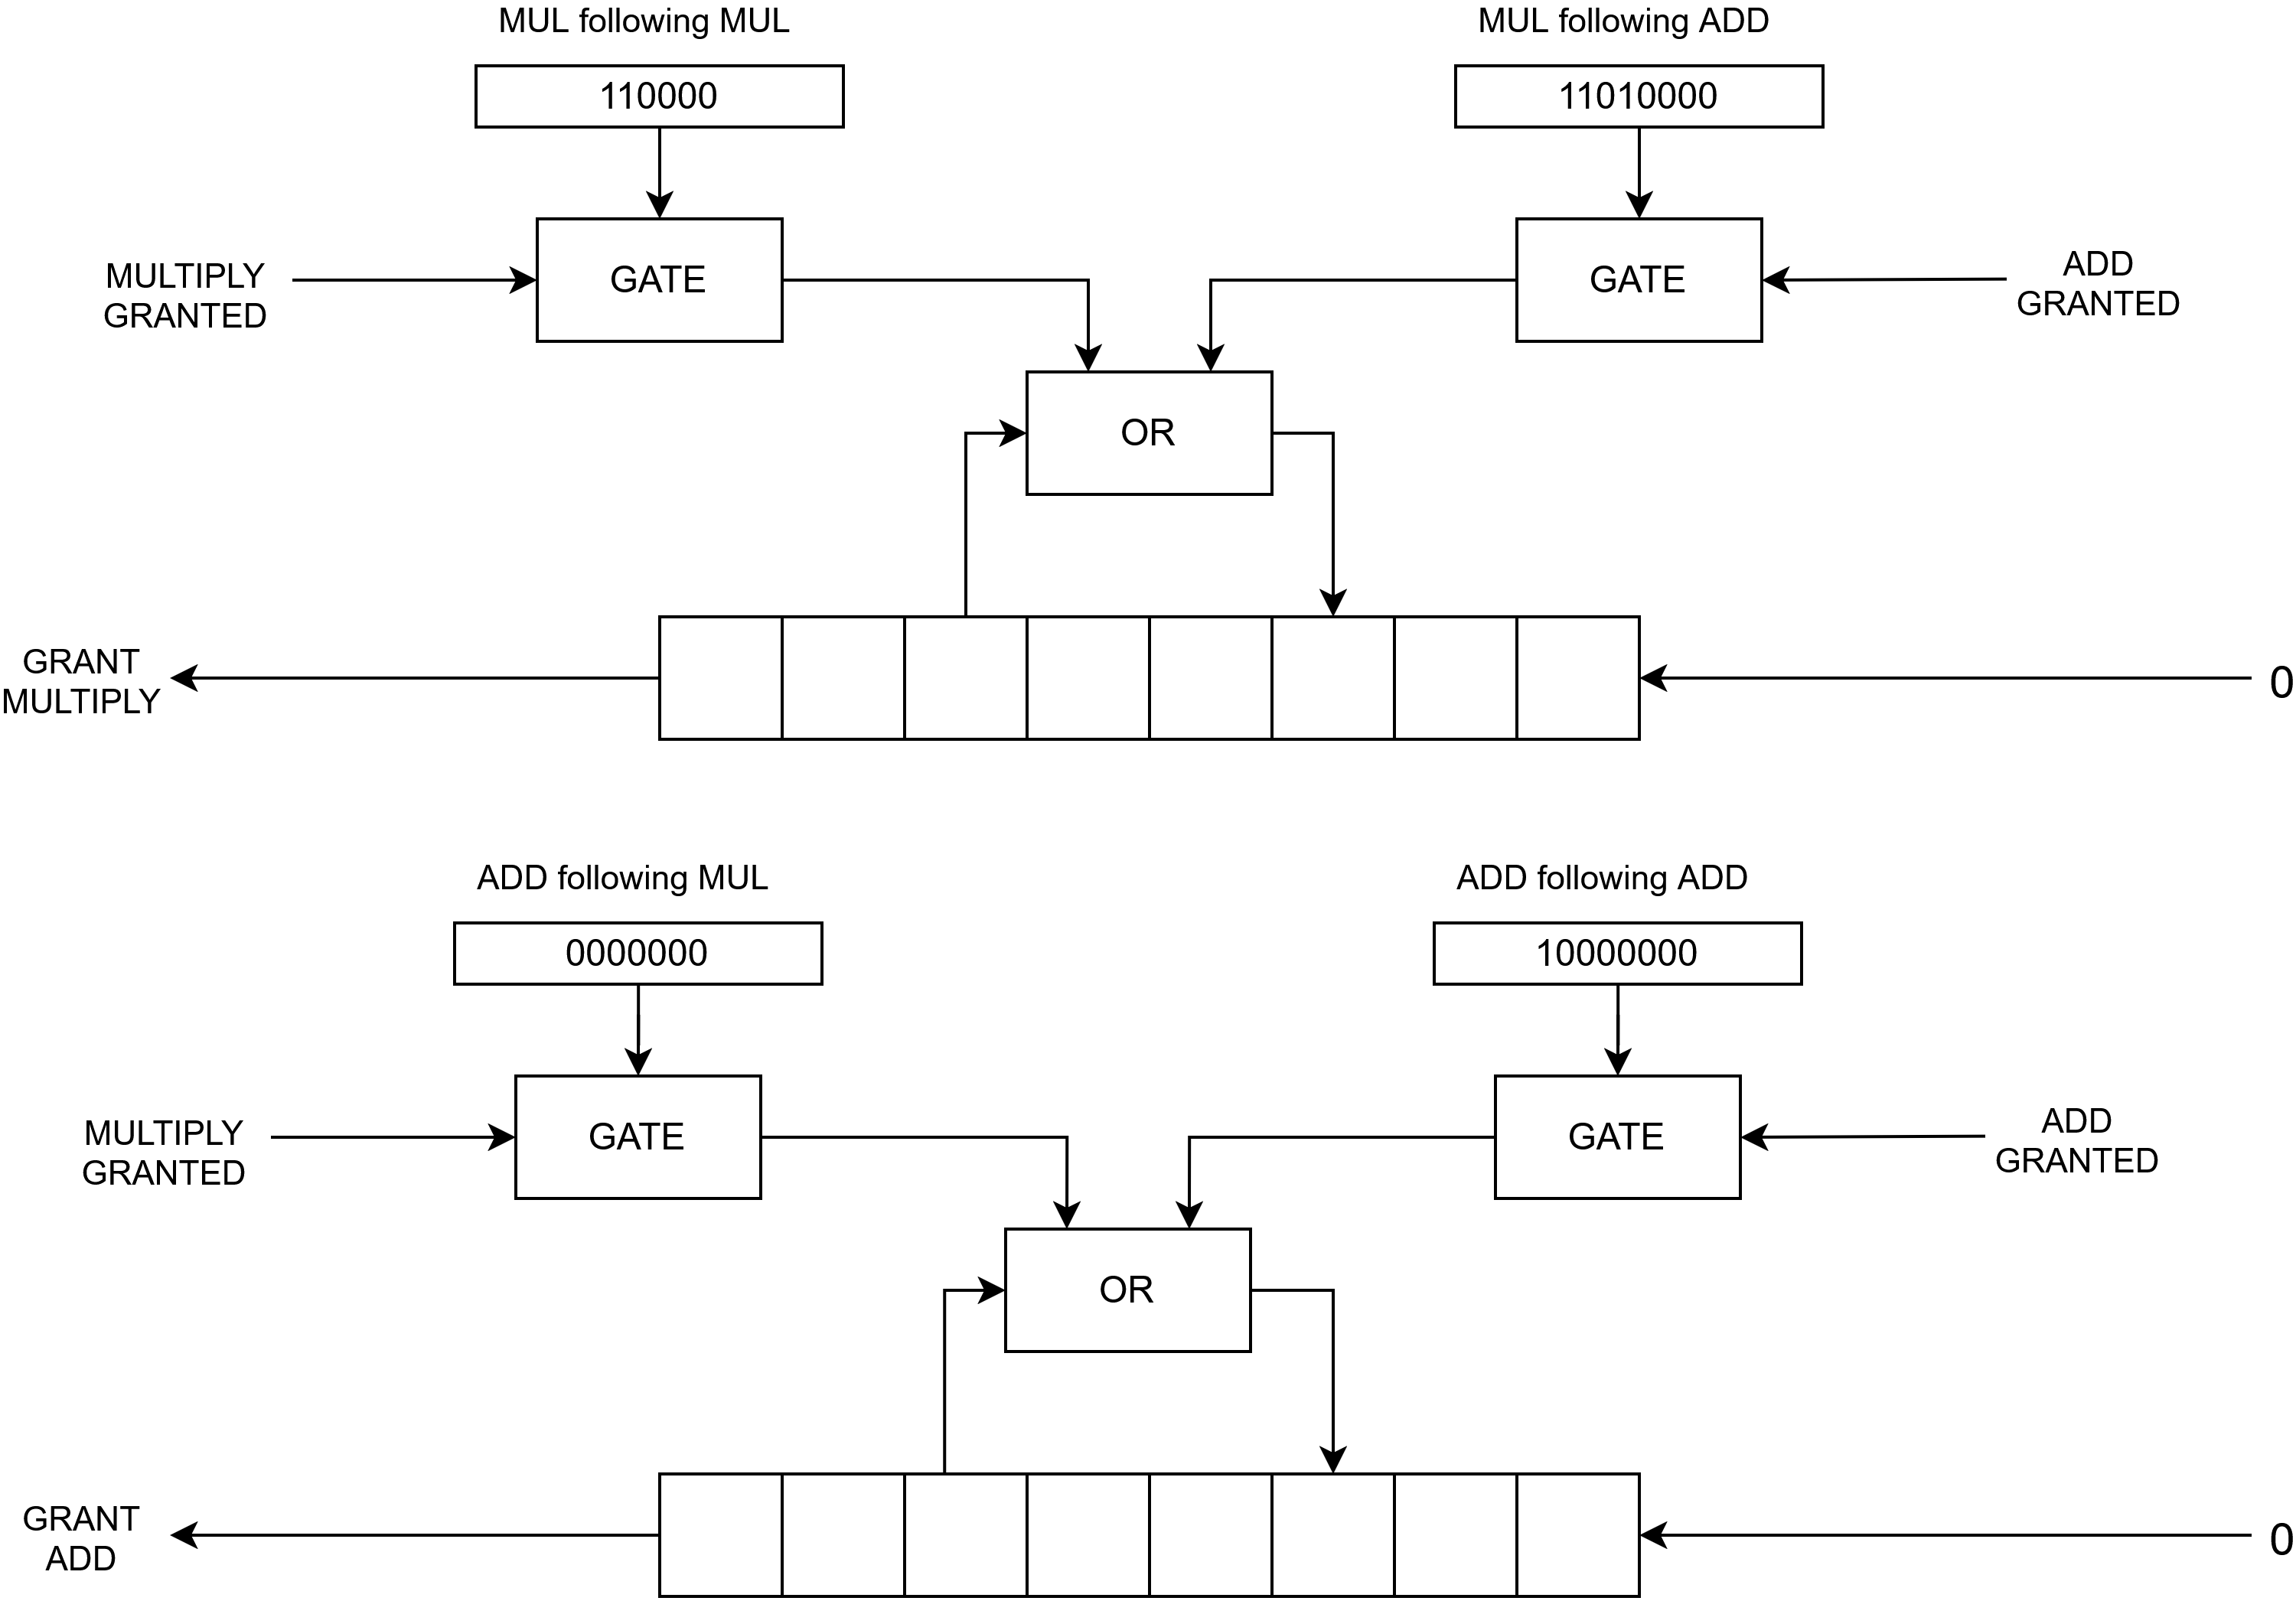
\includegraphics[width=0.7\linewidth]{img/superscalari_collisioni.png}
    \caption{Hardware per la gestione delle collisioni.}
    \label{fig:hardware-coll}
\end{figure}
In particolare, il registro a scorrimento fa proseguire la "storia" delle istruzioni, mentre la OR "unisce" la storia precedente con la nuova. Quindi, la OR garantisce che non ci sia collisione né con l'istruzione che stiamo aggiungendo, né con la storia di istruzioni precedenti. \MakeUppercase{è} fondamentale notare come la struttura sia suddivisa in due parti, quella superiore che riguarda soltanto la moltiplicazione, e quella inferiore che invece riguarda l'addizione.
\\
\\
Un tale tipo di soluzione hardware per la gestione delle collisioni è tipica dei sistemi \textbf{DSP} (Digital Signal Processor), come quelli usati per audio, video, telecomunicazioni. In particolare, il suo utilizzo permette di schedulare le istruzioni nel modo più efficiente possibile evitando stalli o rallentamenti.